\documentclass[10pt,aspectratio=169]{beamer}

% All the boilerplate is in deslides.sty
\usepackage{deslides}

\author{Ji\v{r}\'i Lebl}

\institute[OSU]{%
Oklahoma State University%
%Departemento pri Matematiko de Oklahoma {\^S}tata Universitato%
}

\title{25. Transforms of derivatives and ODEs, part 1\\(Notes on Diffy Qs, 6.2)}

\date{}

\begin{document}

\begin{frame}
\titlepage

%\bigskip

\begin{center}
The textbook: \url{https://www.jirka.org/diffyqs/}
\end{center}
\end{frame}

\begin{frame}
To solve ODEs with Laplace, we need to know how derivatives transform.

\medskip
\pause

Suppose $g(t)$ is a differentiable function of exponential order:

\medskip
\pause

$\lvert g(t) \rvert \leq M e^{ct}$ for some
$M$ and $c$,
\qquad
$\mathcal{L} \bigl\{ g(t) \bigr\}$ exists,
\quad
and
\qquad
 $\lim\limits_{t\to\infty} e^{-st}g(t) = 0$ when $s > c$.

\pause
\[
\mathcal{L} \bigl\{ g'(t) \bigr\}
\pause
=
\int_0^\infty
e^{-st}
g'(t) \,dt
\pause
=
\Bigl[e^{-st} g(t) \Bigr]_{t=0}^\infty
-
\int_0^\infty
(-s)\,
e^{-st}
g(t) \,dt
\pause
=
-g(0) + s \mathcal{L} \bigl\{ g(t) \bigr\} .
\]
\pause

Rinse and repeat for higher derivatives:
\begin{center}
\begin{tabular}{@{}ll@{}}
\toprule
$f(t)$ & $\mathcal{L} \bigl\{ f(t) \bigr\} = F(s)$ \\
\midrule
$g'(t)$ & $sG(s)-g(0)$ \\[4pt]
$g''(t)$ & $s^2G(s)-sg(0)-g'(0)$ \\[4pt]
$g'''(t)$ & $s^3G(s)-s^2g(0)-sg'(0)-g''(0)$ \\[4pt]
\bottomrule
\end{tabular}
\end{center}
\pause
Notice: $G(s)$ is never differentiated, just multiplied by
$s$.

\end{frame}

\begin{frame}
\textbf{Example:}
Consider
\qquad
$x''(t) + x(t) = \cos (2t), \quad x(0) = 0, \quad x'(0) = 1$.

\medskip
\pause

Laplace the equation and write $X(s)$ for $\mathcal{L}\bigl\{x(t)\bigr\}$:
\[
\mathcal{L} \bigl\{ x''(t) + x(t) \bigr\}
= \mathcal{L} \bigl\{ \cos (2t) \bigr\} ,
\pause
\quad
\Rightarrow
\quad
\underbrace{s^2 X(s) -sx(0)-x'(0)}_{\mathcal{L}\{x''(t)\}}
+ \underbrace{X(s)}_{\mathcal{L}\{x''(t)\}}
= \frac{s}{s^2 + 4} .
\]
\pause
Plug in $x(0)=0$ and $x'(0)=1$:
\[
s^2 X(s) -1 + X(s) = \dfrac{s}{s^2 + 4}
\]
\pause
Solve for $X(s)$:
\[
X(s) = \frac{s}{(s^2+1)(s^2 + 4)} + \frac{1}{s^2+1} .
\]
\pause
Use partial fractions (exercise):
\[
X(s) =\frac{1}{3} \, \frac{s}{s^2+1} - 
\frac{1}{3}\, \frac{s}{s^2+4} + \frac{1}{s^2+1} .
\]
\pause
Take the inverse Laplace transform:
\[
x(t) =\frac{1}{3}  \cos (t) -
\frac{1}{3} \cos (2t) + \sin (t) .
\]
\end{frame}

\begin{frame}
So the procedure for constant coefficient linear ODEs is simple:

\begin{enumerate}
\item
\pause
Transform the equation (the equation becomes algebraic):
\\
$x(t)\phantom{{}''}$ \quad $\to$ \quad $X(s)$,
\\
$x'(t)\phantom{{}'}$ \quad $\to$ \quad $sX(s)-x(0)$,
\\
$x''(t)$ \quad $\to$ \quad $s^2X(s)-s x(0) - x'(0)$,
\\
etc.
\item
\pause
Plug in the initial conditions.
\item
\pause
Solve for $X(s)$.
\item
\pause
Compute $x(t) = \mathcal{L}^{-1} \bigl\{ X(s) \bigr\}$.
\end{enumerate}

\medskip
\pause

\textbf{Remark 1:} To be useful, everything in sight
(namely the right hand side, the input) must have
a Laplace transform.  E.g., won't work for $x''+x=\tan(t)$.

\medskip
\pause

\textbf{Remark 2:} On the other hand, Laplace can solve equations
with many right hand sides (inputs) that the other techniques have no chance
of handling.
\end{frame}

\begin{frame}
One type of function Laplace is very good at handling are functions defined
piecewise.  Here's where Heaviside comes in:
\[
u(t) =
\begin{cases}
0 & \text{if } \; t < 0 , \\ 
1 & \text{if } \; t \geq 0 .
\end{cases}
\hspace*{3in}
\]
\vspace*{-0.69in}

\hfill
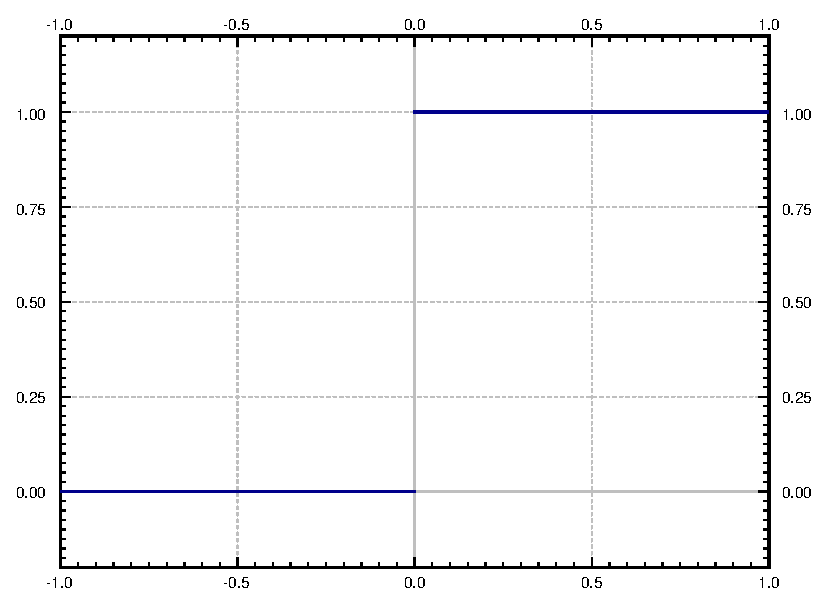
\includegraphics[width=3.0in]{../figures/lt-heaviside}

\pause
\vspace*{-1.50in}

Most commonly used as
\[
u(t-a) =
\begin{cases}
0 & \text{if } \; t < a , \\ 
1 & \text{if } \; t \geq a .
\end{cases}
\hspace*{3in}
\]
\pause
\textbf{Example:}
Suppose:
\begin{equation*}
f(t) =
\begin{cases}
0 & \text{if } \; t < \pi , \\ 
\sin t & \text{if } \; t \geq \pi .
\end{cases}
\hspace*{3in}
\end{equation*}
\pause
Using Heaviside,
you could write $f$ as: \quad $f(t) = u(t - \pi) \, \sin t$.
\end{frame}

\begin{frame}
A step function that is $0$ everywhere except on $[1,2)$ where it is 1
can be written as
\[
u(t - 1) - u(t-2) .
\]
\pause
Useful for piecewise defined functions.  E.g.,
\[
f(t) =
\begin{cases}
t & \text{if } \; t \in [0,1) , \\ 
-t+2 & \text{if } \; t \in [1,2), \\
0 & \text{otherwise} .
\end{cases}
\]
becomes
\[
f(t) = t \, \bigl( u(t) - u(t-1) \bigr) + 
(-t+2) \, \bigl( u(t - 1) - u(t-2) \bigr) .
\]
\pause
We Laplace transform such functions using the \emph{second shifting property}:
\[
\mathcal{L} \bigl\{ f(t-a) \, u(t-a) \bigr\}
= e^{-as} \mathcal{L} \bigl\{ f(t) \bigr\} .
\]
\pause
\textbf{Example:}
\[
\mathcal{L} \bigl\{ t \, u(t-1) \bigr\}
\pause
=
\mathcal{L} \bigl\{ \bigl( (t-1) + 1\bigr) \, u(t-1) \bigr\}
\pause
= e^{-as} \mathcal{L} \bigl\{ t+1 \bigr\}
\pause
= e^{-as} \left(\frac{1}{s^2} + \frac{1}{s} \right)
.
\]
\end{frame}

\begin{frame}
\textbf{Example:}
Consider the mass-spring setup
\begin{equation*}
x''(t) + x(t) = f(t) , \quad x(0) = 0, \quad x'(0) = 0,
\end{equation*}
where $f(t) = 1$ if $1 \leq t < 5$ and zero otherwise.

\pause
\medskip

E.g., a rocket motor attached to the mass is fired for 4 seconds starting at
$t=1$. \pause  Or an RLC circuit where the voltage is raised
at a constant rate for 4 seconds starting at $t=1$ held steady 
again starting at $t=5$.

\pause
\medskip

Write $f(t) = u(t-1) - u(t-5)$ and transform the equation
\[
x''(t) + x'(t) = 
u(t-1) - u(t-5)
\qquad
\Rightarrow
\qquad
s^2 X(s) + X(s) = \frac{e^{-s}}{s} - \frac{e^{-5s}}{s} .
\]
\pause
Solve for $X(s)$:
\[
X(s) = \frac{e^{-s}}{s(s^2+1)} - \frac{e^{-5s}}{s(s^2+1)} .
\]
\pause
\textbf{Exercise} (need to use partial fractions)\textbf{:}
\begin{equation*}
{\mathcal{L}}^{-1} \left\{ \frac{1}{s(s^2+1)} \right\}
= 1 - \cos t .
\end{equation*}
\end{frame}

\begin{frame}
$\mathcal{L} \{ 1 - \cos t  \} = \frac{1}{s(s^2+1)}$ and the
second shifting property (in reverse) says
\[
{\mathcal{L}}^{-1} \left\{ \frac{e^{-s}}{s(s^2+1)} \right\}
\pause
=
{\mathcal{L}}^{-1} \bigl\{
e^{-s}
\mathcal{L} \{ 1 - \cos t \}
\bigr\}
\pause
=
\bigl( 1 - \cos (t-1) \bigr) \, u(t-1) .
\]
\pause
Similarly,
\[
{\mathcal{L}}^{-1} \left\{ \frac{e^{-5s}}{s(s^2+1)} \right\}
=
{\mathcal{L}}^{-1} \bigl\{
e^{-5s}
\mathcal{L} \{ 1 - \cos t \}
\bigr\}
=
\bigl( 1 - \cos (t-5) \bigr) \, u(t-5) .
\]
\pause
Hence, as

\bigskip

$\quad
X(s) = \dfrac{e^{-s}}{s(s^2+1)} - \dfrac{e^{-5s}}{s(s^2+1)}$ ,

\bigskip
\pause

we have

\medskip

$
\quad
x(t) = 
\bigl( 1 - \cos (t-1) \bigr) \, u(t-1) $

\medskip

$\qquad\qquad {} -
\bigl( 1 - \cos (t-5) \bigr) \, u(t-5)$.

\vspace*{-1.6in}

\hfill
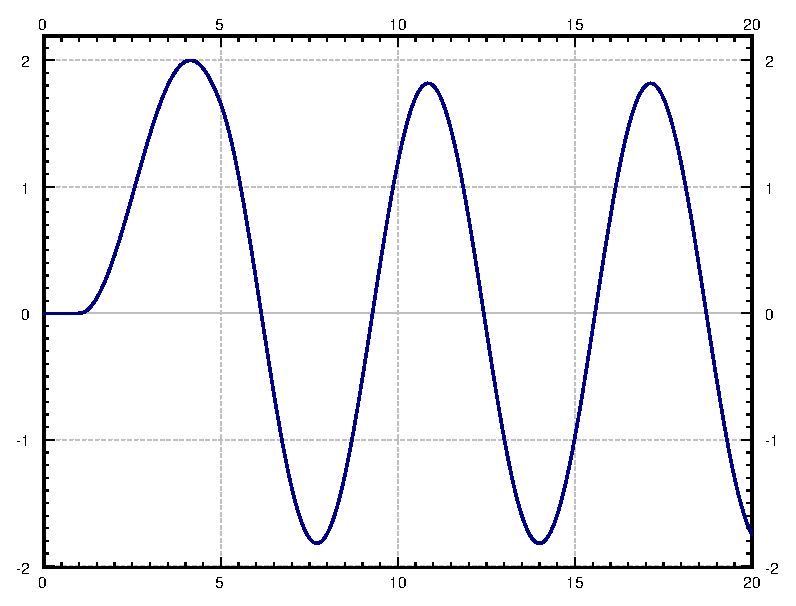
\includegraphics[width=2.5in]{../figures/lt-heavisideex}
\end{frame}


\end{document}
